\documentclass[aspectratio=169]{../latex_main/tntbeamer}  % you can pass all options of the beamer class, e.g., 'handout' or 'aspectratio=43'
\usepackage{dsfont}
\usepackage{bm}
\usepackage[english]{babel}
\usepackage[T1]{fontenc}
%\usepackage[utf8]{inputenc}
\usepackage{graphicx}
\graphicspath{ {./figures/} }
\usepackage{algorithm}
\usepackage[ruled,vlined,algo2e,linesnumbered]{algorithm2e}
\usepackage{hyperref}
\usepackage{booktabs}
\usepackage{mathtools}

\usepackage{amsmath,amssymb}

\DeclareMathOperator*{\argmax}{arg\,max}
\DeclareMathOperator*{\argmin}{arg\,min}

\usepackage{amsbsy}
\newcommand{\vect}[1]{\bm{#1}}
%\newcommand{\vect}[1]{\boldsymbol{#1}}

\usepackage{pgfplots}
\pgfplotsset{compat=1.16}
\usepackage{tikz}
\usetikzlibrary{trees} 
\usetikzlibrary{shapes.geometric}
\usetikzlibrary{positioning,shapes,shadows,arrows,calc,mindmap}
\usetikzlibrary{positioning,fadings,through}
\usetikzlibrary{decorations.pathreplacing}
\usetikzlibrary{intersections}
\pgfdeclarelayer{background}
\pgfdeclarelayer{foreground}
\pgfsetlayers{background,main,foreground}
\tikzstyle{activity}=[rectangle, draw=black, rounded corners, text centered, text width=8em]
\tikzstyle{data}=[rectangle, draw=black, text centered, text width=8em]
\tikzstyle{myarrow}=[->, thick, draw=black]

% Define the layers to draw the diagram
\pgfdeclarelayer{background}
\pgfdeclarelayer{foreground}
\pgfsetlayers{background,main,foreground}

% Requires XeLaTeX or LuaLaTeX
%\usepackage{unicode-math}

\usepackage{fontspec}
%\setsansfont{Arial}
\setsansfont{RotisSansSerifStd}[ 
Path=../latex_main/fonts/,
Extension = .otf,
UprightFont = *-Regular,  % or *-Light
BoldFont = *-ExtraBold,  % or *-Bold
ItalicFont = *-Italic
]
\setmonofont{Cascadia Mono}[
Scale=0.8
]

% scale factor adapted; mathrm font added (Benjamin Spitschan @TNT, 2021-06-01)
%\setmathfont[Scale=1.05]{Libertinus Math}
%\setmathrm[Scale=1.05]{Libertinus Math}

% other available math fonts are (not exhaustive)
% Latin Modern Math
% XITS Math
% Libertinus Math
% Asana Math
% Fira Math
% TeX Gyre Pagella Math
% TeX Gyre Bonum Math
% TeX Gyre Schola Math
% TeX Gyre Termes Math

% Literature References
\newcommand{\lit}[2]{\href{#2}{\footnotesize\color{black!60}[#1]}}

%%% Beamer Customization
%----------------------------------------------------------------------
% (Don't) Show sections in frame header. Options: 'sections', 'sections light', empty
\setbeamertemplate{headline}{empty}

% Add header logo for normal frames
\setheaderimage{
	% 
\includegraphics[height=\logoheight]{figures/TNT_darkv4.pdf}
	
\includegraphics[height=\logoheight]{../latex_main/figures/luh_logo_rgb_0_80_155.pdf}
	% 
\includegraphics[height=\logoheight]{figures/logo_tntluh.pdf}
}

% Header logo for title page
\settitleheaderimage{
	% 
\includegraphics[height=\logoheight]{figures/TNT_darkv4.pdf}
	
\includegraphics[height=\logoheight]{../latex_main/figures/luh_logo_rgb_0_80_155.pdf}
	% 
\includegraphics[height=\logoheight]{figures/logo_tntluh.pdf}
}

% Title page: tntdefault 
\setbeamertemplate{title page}[tntdefault]  % or luhstyle
% Add optional title image here
%\addtitlepageimagedefault{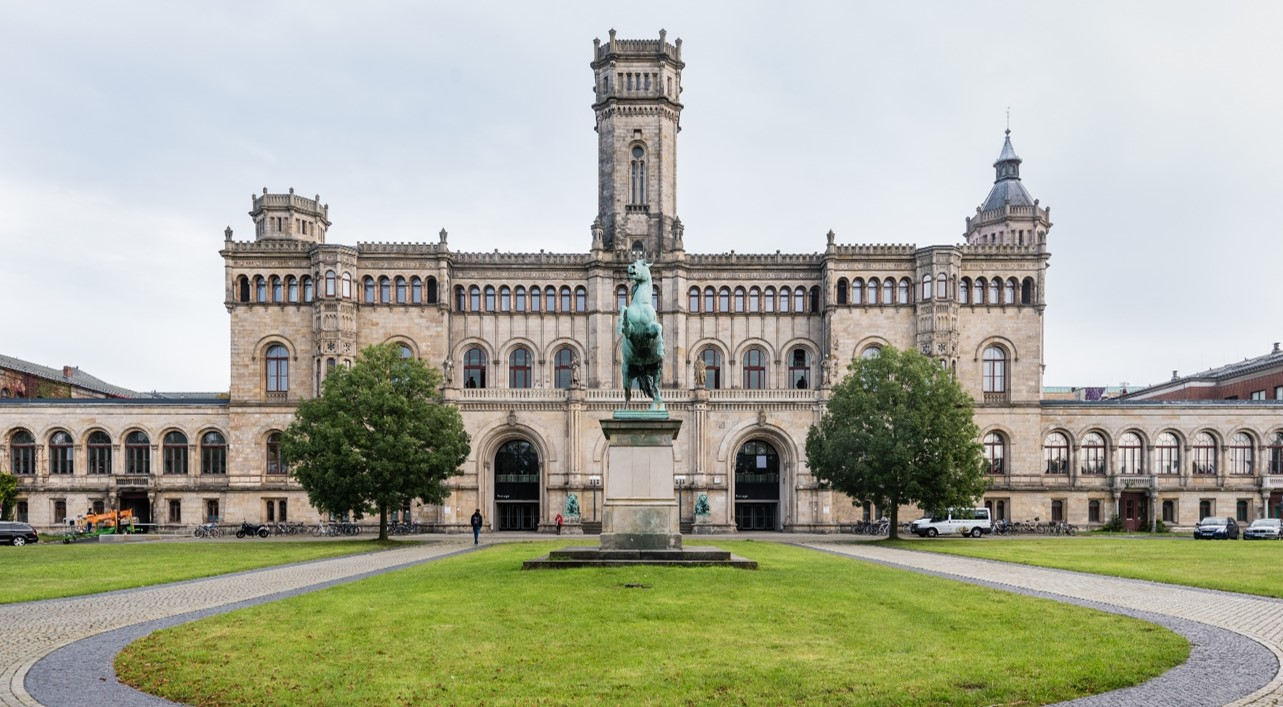
\includegraphics[width=0.65\textwidth]{figures/luh_default_presentation_title_image.jpg}}

% Title page: luhstyle
% \setbeamertemplate{title page}[luhstyle]
% % Add optional title image here
% \addtitlepageimage{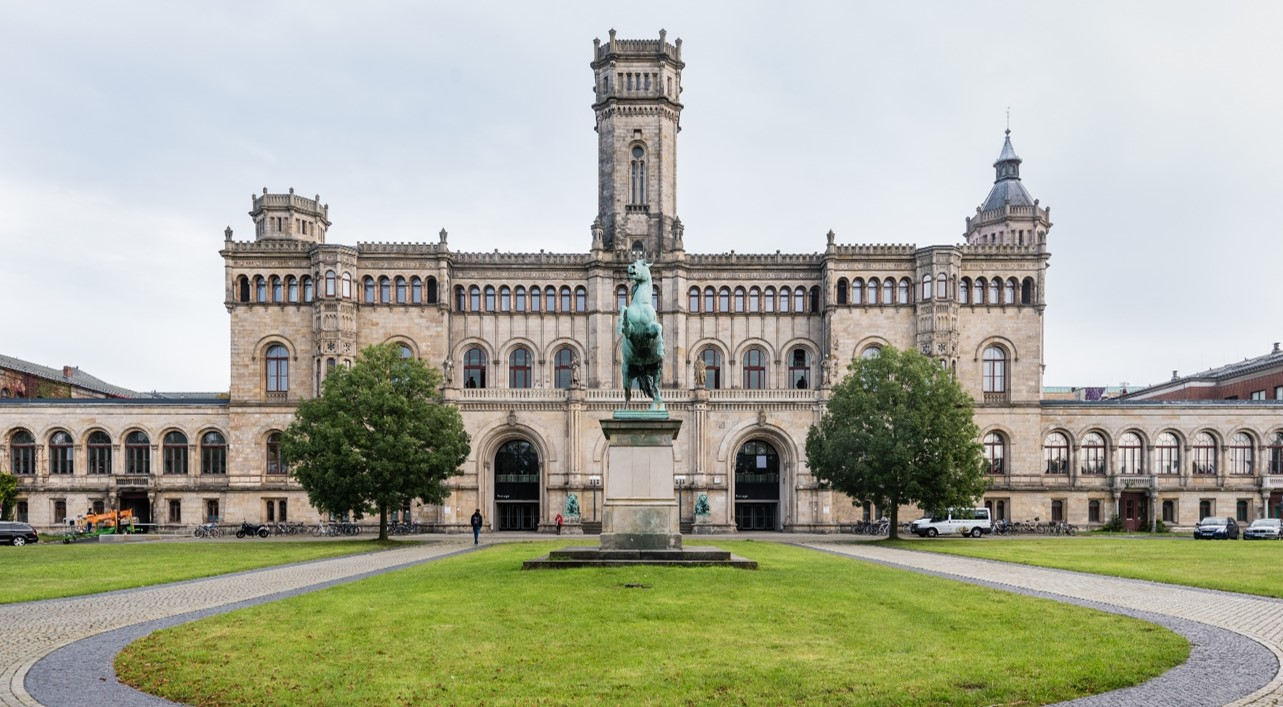
\includegraphics[width=0.75\textwidth]{figures/luh_default_presentation_title_image.jpg}}

\author[Abedjan \& Lindauer]{Ziawasch Abedjan \& Marius Lindauer\\[1em]
	
\includegraphics[height=\logoheight]{../latex_main/figures/luh_logo_rgb_0_80_155.pdf}\qquad
	
\includegraphics[height=\logoheight]{../latex_main/figures/DBIS_Kurzlogo.png}\qquad

\includegraphics[height=\logoheight]{../latex_main/figures/TNT_darkv4}\qquad

\includegraphics[height=\logoheight]{../latex_main/figures/L3S.jpg}	}
\date{Summer Term 2022; \hspace{0.5em} {
\includegraphics[height=1.5em]{../latex_main/figures/Cc-by-nc-sa_icon.svg.png}}; based on \href{https://ds100.org/fa21/}{[DS100]}
}


%%% Custom Packages
%----------------------------------------------------------------------
% Create dummy content
\usepackage{blindtext}

% Adds a frame with the current page layout. Just call \layout inside of a frame.
\usepackage{layout}


%%% Macros
%\renewcommand{\vec}[1]{\mathbf{#1}}
% \usepackage{bm}
%\let\vecb\bm

\title[CV, Reg \& AutoML]{DS: Cross-Validation, Regularization \& AutoML}
\subtitle{AutoML: Basics}

\graphicspath{ {./figure/} }
%\institute{}


\begin{document}
\maketitle

\begin{frame}[c]{Problem of Hyperparameters}
	
	\begin{itemize}
	    \item We have seen that algorithms have important hyperparameters
	    \item Depending on your hyperparameter configuration, your model might learn only noise, will learn a constant model or maybe even achieve state-of-the-art performance 
	    \item In fact, many ML algorithms are fairly brittle regarding their hyperparameter configuration
	    \medskip
	    \item Since we cannot directly learn the hyperparameter configuration from data, we have tune somehow differently
	    \item Manual hyperparameter optimization?
	    \begin{itemize}
	        \item tedious, error-prone, time-consuming
	        \item Requires years of expertise
	    \end{itemize}
	    \smallskip
	    \item Simply choosing default settings?
	    \begin{itemize}
	        \item Developers of algorithms often tuned the hyperparameters on a limited set of datasets
	        \item[$\leadsto$] might work well on your dataset or might fail
	    \end{itemize}
	    \item[$\leadsto$] Can we automate this process?
	\end{itemize}
	
\end{frame}
%-----------------------------------------------------------------------
%----------------------------------------------------------------------
\begin{frame}[c]{What are Hyperparameters in ML?}
	
	\begin{itemize}
	    \item ...
	\end{itemize}
	
\end{frame}
%-----------------------------------------------------------------------
%----------------------------------------------------------------------
\begin{frame}[c]{What are Hyperparameters in ML?}
	
	\begin{itemize}
	    \item Regularization strength
	    \item Complexity of model (e.g., degree of polynomial)
	    \smallskip
	    \item Which regression model to use (e.g., lasso or ridge regression)
	    \item Which data reduction technique to use (e.g., feature selection or PCA)
	    \item Which feature normalization technique to use (e.g., standardization or min-max scaling)
	    \smallskip
	    \item Learning rate in Deep Learning
	    \item Architecture of your neural network
	    \item \ldots
	\end{itemize}
	
	\bigskip
	\alert{Warning:} The correct configuration of your hyperparameters depends on your dataset at hand.
	
\end{frame}
%-----------------------------------------------------------------------
%----------------------------------------------------------------------
\begin{frame}[c]{Effect of Hyperparameter Optimization}
	
	\centering
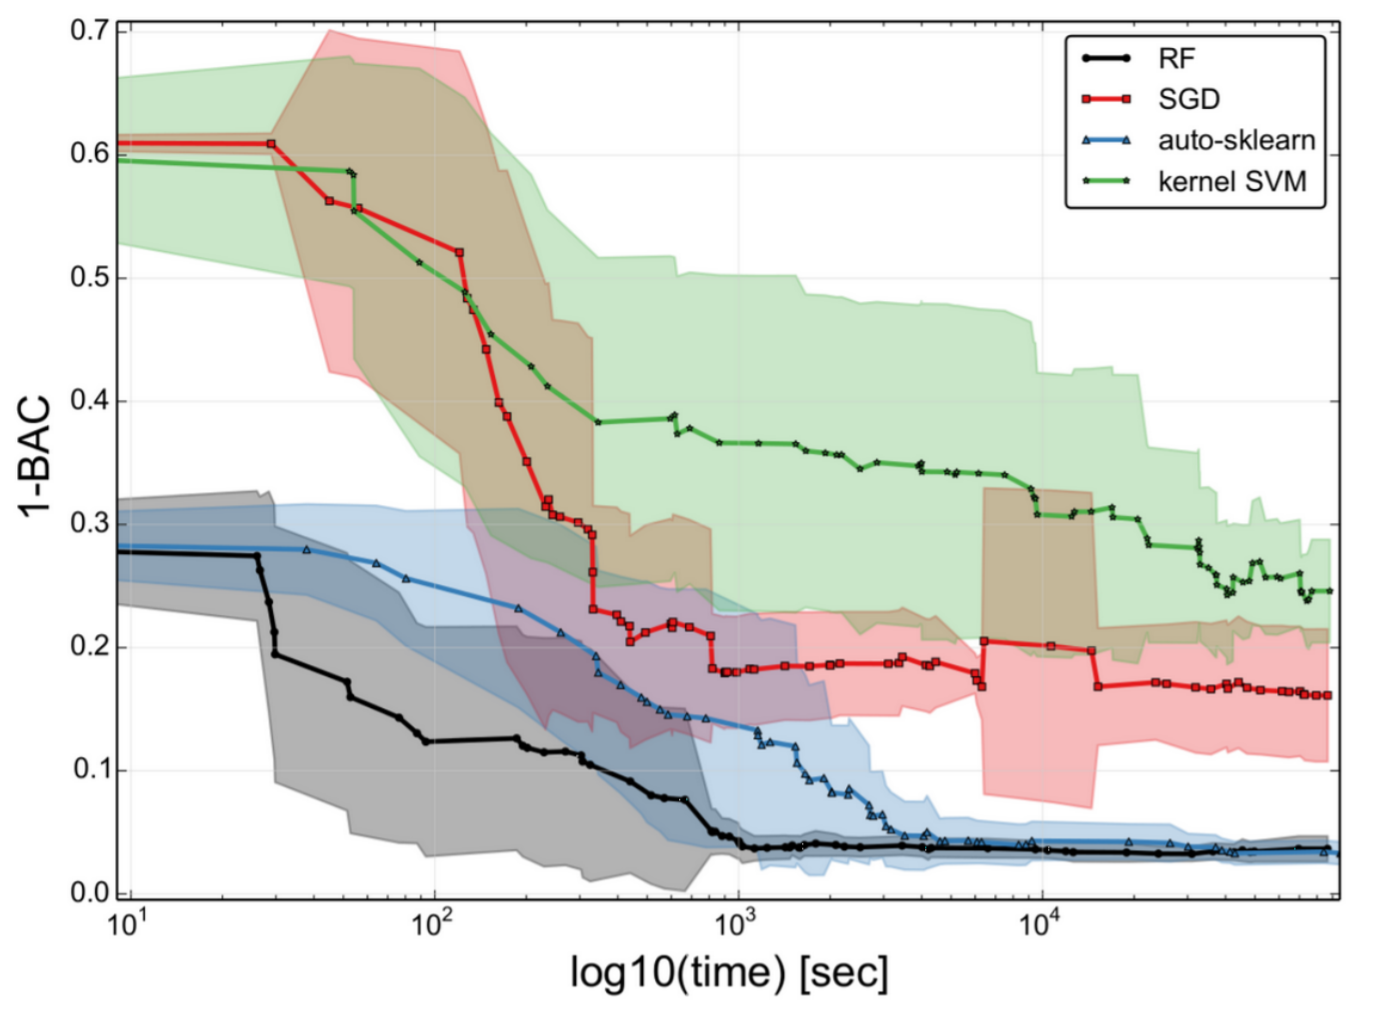
\includegraphics[width=0.63\textwidth]{09_cv_reg_auto/figure/image12.png}
	
\end{frame}
%-----------------------------------------------------------------------
\begin{frame}[c]{Grid Search vs. Random Search}

\vspace{-1em}
\begin{itemize}
    \item Let's tune 2 hyperparameters 
    \item Plotting the samples of hyperparameter configurations for grid search and random search
    \item On each axis, we see the effect of each hyperparameter on the performance
\end{itemize}

\centering
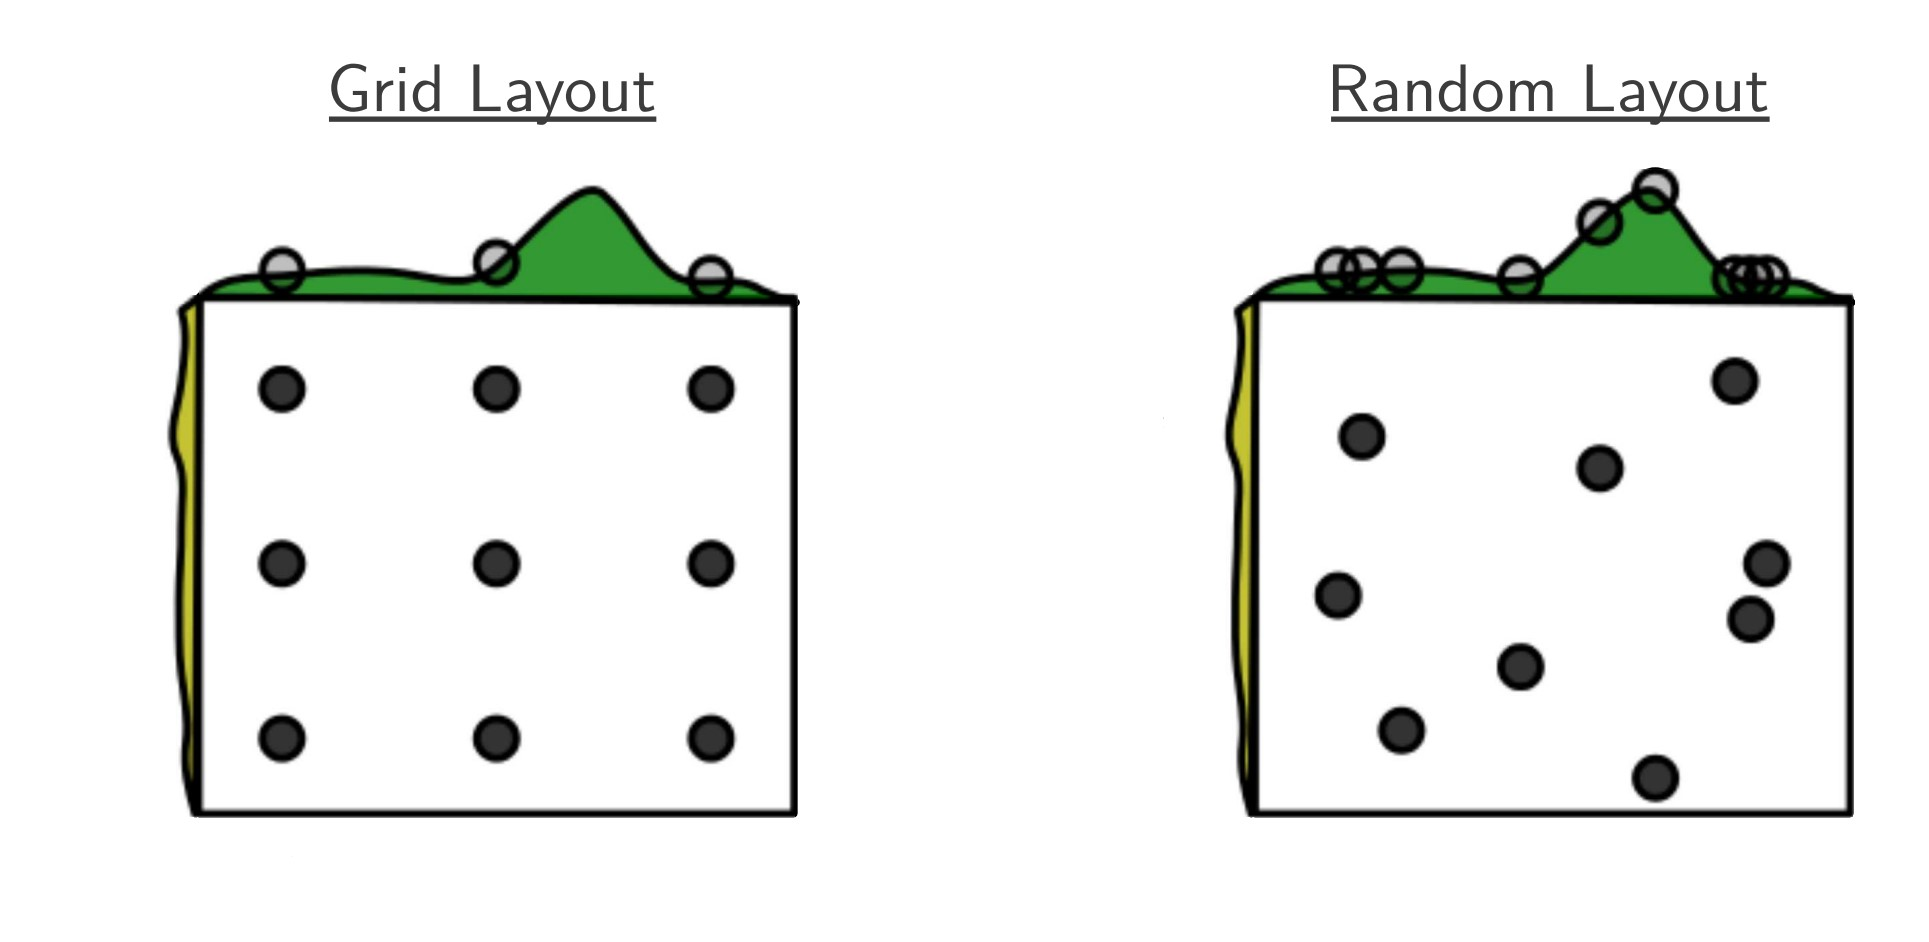
\includegraphics[width=.72\textwidth]{figure/grid_random.jpg}

\footnotesize
[\href{https://www.jmlr.org/papers/volume13/bergstra12a/bergstra12a.pdf}{Bergstra and Bengio 2012}]


\end{frame}
%-----------------------------------------------------------------------
%-----------------------------------------------------------------------
\begin{frame}[c]{Grid Search vs. Random Search}
	
\begin{itemize}
    \item Grid Search:
    \begin{itemize}
        \item[+] Structured study
        \item[-] Requires discretization (from an expert)
        \item[-] Doesn't scale well to high dimensions
        \item[-] Cannot be interrupted mid-way
    \end{itemize}
    \item Random Search
    \begin{itemize}
        \item[+/-] Less structured
        \item[+] Works better if effective dimensionality is low 
        \item[+] Better anytime behavior
        \item[+] Easy to add more points later on
        \item[-] Still very inefficient
    \end{itemize}
\end{itemize}
\end{frame}
%-----------------------------------------------------------------------

\end{document}